\documentclass[tikz,border=10pt]{standalone}
\usepackage{amsmath}
\usepackage{amssymb}
\definecolor{mantis}{RGB}{0, 105, 62}
\begin{document}
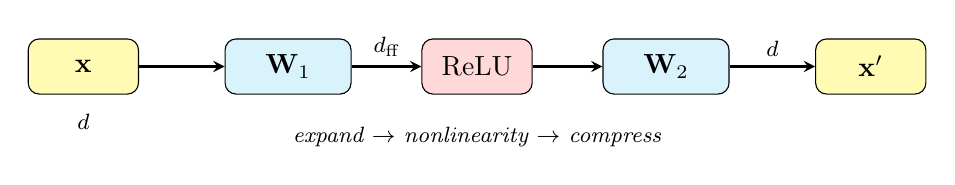
\begin{tikzpicture}[>=stealth]
    \node[draw, rounded corners, fill=yellow!30, minimum width=1.4cm, minimum height=0.7cm] (x) at (0,0) {$\mathbf{x}$};
    \node[draw, rounded corners, fill=cyan!15, minimum width=1.6cm, minimum height=0.7cm] (W1) at (2.6,0) {$\mathbf{W}_1$};
    \node[draw, rounded corners, fill=red!15, minimum width=1.4cm, minimum height=0.7cm] (relu) at (5,0) {ReLU};
    \node[draw, rounded corners, fill=cyan!15, minimum width=1.6cm, minimum height=0.7cm] (W2) at (7.4,0) {$\mathbf{W}_2$};
    \node[draw, rounded corners, fill=yellow!30, minimum width=1.4cm, minimum height=0.7cm] (out) at (10,0) {$\mathbf{x}'$};
    \draw[->, thick] (x) -- (W1);
    \draw[->, thick] (W1) -- (relu) node[midway, above, font=\footnotesize] {$d_{\text{ff}}$};
    \draw[->, thick] (relu) -- (W2);
    \draw[->, thick] (W2) -- (out) node[midway, above, font=\footnotesize] {$d$};
    \node[font=\footnotesize] at (0,-0.7) {$d$};
    \node[font=\footnotesize\itshape] at (5,-0.9) {expand $\to$ nonlinearity $\to$ compress};
\end{tikzpicture}
\end{document}
